%!TEX root = ../thesis.tex
% appendix section 2

\chapter{High-pressure chamber system}
\label{sec:ap2}

\section{Modularized system}
\label{sec:ap2-1}

\begin{figure}[ht!]
\centering
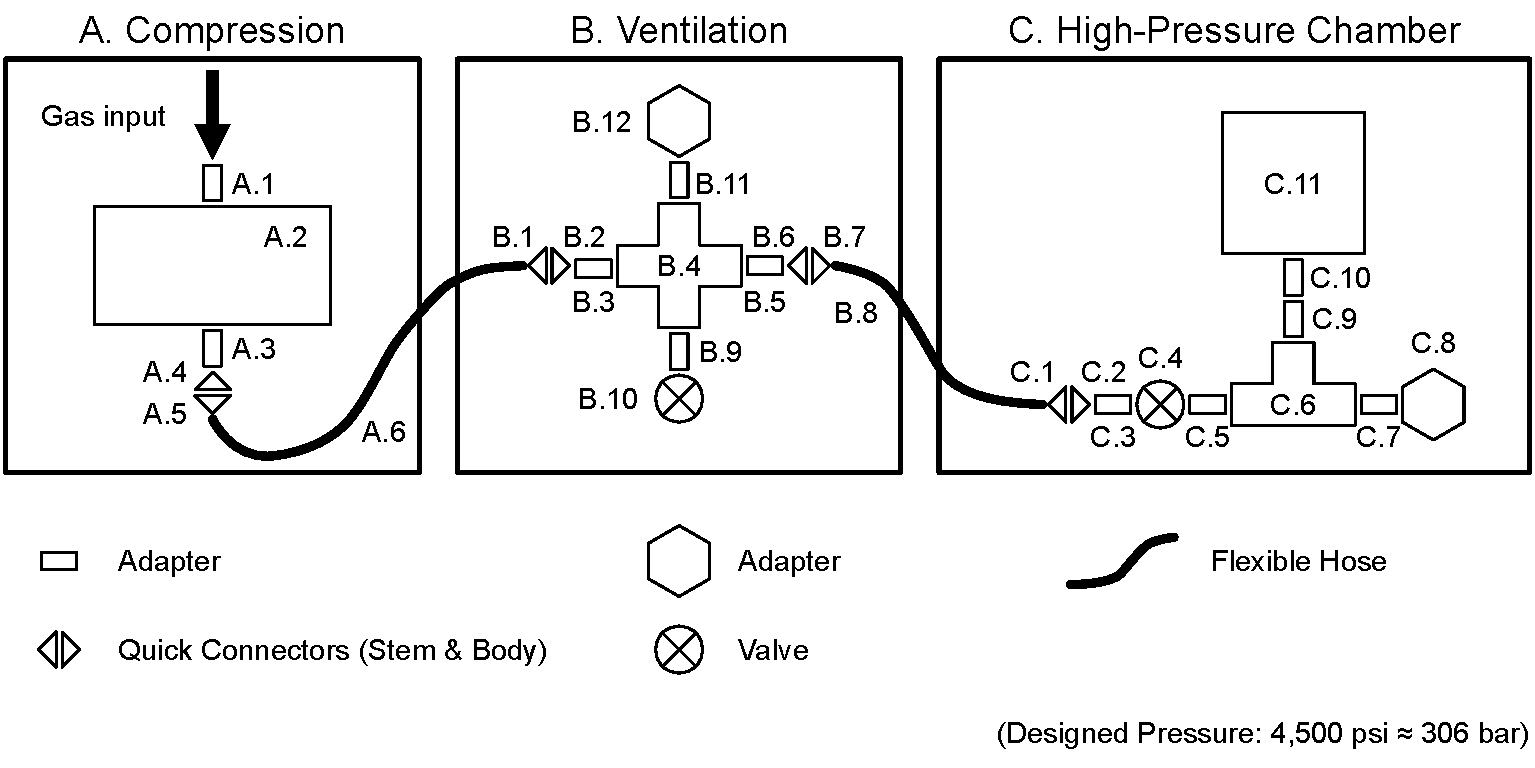
\includegraphics[width=130mm]{figures/ap2/system/moduleSystem.pdf}
\caption{Modularized chamber system. The high-pressure system is designed for the operation up to $4,500 \text{ psi} \approx 306 \text{ bar}$. The information of the parts is listed in Table.\ref{table:partList}.}
\label{fig:moduleSystem}
\end{figure}

The reciprocating compressor has a cycling frequency of about $4.1 \text{ Hz}$ and a throughput of about $6.8 \text{ cm}^{3} \cdot \text{cycle}^{-1}$ (under standard conditions). A pair of bendable stainless-steel hoses (Swagelok SS-FX4TA4TA4) is installed to add flexibility to the system. Quick-connect adapters (SS-QF4-S, SS-QF4-B) are placed at the junctions, which modularize the system and thereby make it possible to carry the chamber after compression \ref{fig:moduleSystem}. The cubic-shaped stainless-steel chamber (side length: $65 \text{ mm}$) is computer numerical control (CNC) machined to make six threading ports (1 1/16-12-UN) with O-ring grooves (SAE J1926-1). One of the ports is used as the gas entrance, and sight windows are installed on the other ports. The sight windows, made of sapphire glass (thickness: $7.2 \text{ mm}$) and bonded in the stainless-steel housing, has a clear aperture $11.2 \text{ mm}$ in diameter (Rayotek 101117C). Two different pressure sensors, one with a digital display (Keller LEO2) and the other with an analog voltage output (Tival Sensors TST-20) are installed to monitor the pressure for safety. A thermocouple (Fluke 80PK-27) is used to measure the temperature of the expanding fluids.

\begin{table}[h!]
\footnotesize
\centering
\begin{tabular}{lllll}
\hline \hline
Label & Name        & Company  & Part \#       & Description                                                    \\ \hline \hline
A.1   & Adapter     & Sang-A   & GPC 0602       & $1/4"$ NPT (M) to 6 mm tube                                        \\
A.2   & Compressor  & Shoebox  & Shoebox MAX    & Compressor 4,500 psi                           \\
A.3   & Adapter     & Unilok   & PNA-0402N      &  $1/8"$ NPT (M) to $1/4"$ NPT (F)                                       \\
A.4   & QC          & Swagelok & SS-QF4-S-4PM   & QF4 (stem) to $1/4"$ NPT(M)                                        \\
A.5   & QC          & Swagelok & SS-QF4-B-400   & QF4 (body) to $1/4"$ lok fitting                                   \\
A.6   & Hose        & Swagelok & SS-FX4TA4TA4   & Stainless steel hose, $1/4"$, 20cm                                 \\
\hline
B.1   & QC          & Swagelok & SS-QF4-B-400   & QF4 (body) to $1/4"$ lok fitting                                   \\
B.2   & QC          & Swagelok & SS-QF4-S-400   & QF4 (stem) to $1/4"$ lok fitting                                   \\
B.3   & Adapter     & FluxLok  & FLPC-0404T     & $1/4"$ port connector                                              \\
B.4   & Cross & Swagelok & SS-400-4       & $1/4"$ lok fitting cross                                           \\
B.5   & Adapter     & FluxLok  & FLPC-0404T     & $1/4"$ port connector                                              \\
B.6   & QC          & Swagelok & SS-QF4-S-400   & QF4 (stem) to $1/4"$ lok fitting                                   \\
B.7   & QC          & Swagelok & SS-QF4-B-400   & QF4 (body) to $1/4"$ lok fitting                                   \\
B.8   & Hose        & Swagelok & SS-FX4TA4TA4   & Stainless steel hose, $1/4"$, 20cm                                 \\
B.9   & Adapter     & FluxLok  & FLMA-04T04R    & $1/4"$ PT (M) to $1/4"$ pipe                                           \\
B.10  & Valve       & Syntek   & STH12C084T2S-H & Solenoid valve 280 bar, $1/4"$ PT (F)                \\
B.11  & Adapter     & Swagelok & SS-4-TA-7-4RJ  & $1/4"$ G (F) to $1/4"$ pipe                           \\
B.12  & Gauge       & Keller   & LEO 2          & Pressure gauge, $1/4"$ G (M) \\
\hline
C.1   & QC          & Swagelok & SS-QF4-B-400   & QF4 (body) to $1/4"$ lok fitting                                   \\
C.2   & QC          & Swagelok & SS-QF4-S-400   & QF4 (stem) to $1/4"$ lok fitting                                   \\
C.3   & Adapter     & FluxLok  & FLPC-0404T     & $1/4"$ port connector                                              \\
C.4   & Valve       & FluxLok  & FL-HBV1-4      & $1/4"$ lok fitting 2 way ball valve      \\
C.5   & Adapter     & FluxLok  & FLPC-0404T     & $1/4"$ port connector                                              \\
C.6   & Tee   & Swagelok & SS-400-3       & $1/4"$ lok fitting tee                                             \\
C.7   & Adapter     & Swagelok & SS-4-TA-7-4RJ  & $1/4"$ G (F) to $1/4"$ pipe                           \\
C.8   & Sensor      & Tival    & TST-20         & Pressure sensor, $1/4"$ PF (M)        \\
C.9   & Adapter     & Swagelok & SS-811-PC-4    & $1/4"$ to $1/4"$ reducing port connector                               \\
C.10  & Adapter     & Swagelok & SS-810-1-12ST  & 1 1/16-12 SAE (M) to $1/4"$ lok fitting                            \\
C.11  & Chamber     &          &                & 6 way 1 1/16-12 SAE (F) \\
\hline \hline
\end{tabular}
\caption{Parts list for the high-pressure chamber system.}
\label{table:partList}
\end{table}

\pagebreak

\section{Chamber leak test}
\label{sec:ap2-2}

The high-pressure chamber can preserve the internal pressure securely for a long time (Fig.\ref{fig:leak}).

\begin{figure}[h!]
\centering
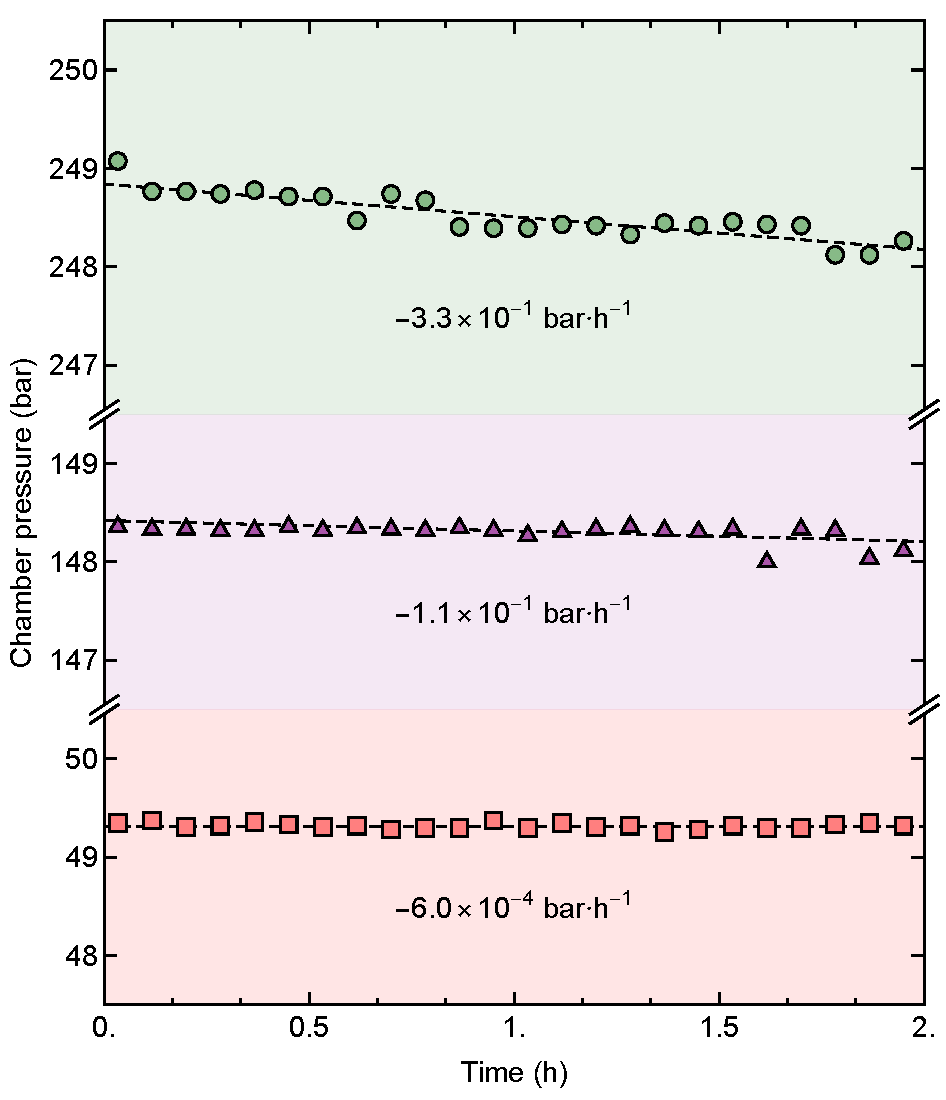
\includegraphics[width=80mm]{figures/ap2/leak/leak.pdf}
\caption{The high-pressure chamber leak test results. The chamber securely preserves the internal pressure for the experimental timescale.}
\label{fig:leak}
\end{figure}
